\documentclass[12pt]{article}
\usepackage[spanish]{babel}
\usepackage{geometry}
\geometry{a4paper, margin=1in}
\usepackage{graphicx}
\usepackage{xcolor}
\usepackage{titlesec}
\usepackage{parskip}
\usepackage{multicol}
\usepackage{cite}

\definecolor{highlight}{RGB}{255, 255, 0}

\titleformat{\section}{\normalfont\Large\bfseries}{\thesection}{1em}{}
\titleformat{\subsection}{\normalfont\large\bfseries}{\thesubsection}{1em}{}

\begin{document}

% Logos
\begin{minipage}{0.45\textwidth}
    
\includegraphics[width=0.4\textwidth]{inFiles/Figures/epnLogo.jpg}
\end{minipage}
\hfill
\begin{minipage}{0.45\textwidth}
    \raggedleft
    
\includegraphics[width=0.4\textwidth]{inFiles/Figures/FIS_logo.jpg}
\end{minipage}

\vspace{0.5cm}

% Títulos principales
\begin{center}
    \textbf{ESCUELA POLITÉCNICA NACIONAL}\\[0.2cm]
    \textbf{FACULTAD DE INGENIERÍA DE SISTEMAS}\\[0.2cm]
    \textbf{INGENIERÍA {\textbf{EN COMPUTACION}}}
\end{center}

\vspace{0.5cm}
\hrule
\vspace{0.5cm}

% Datos principales
\noindent\textbf{PERÍODO ACADÉMICO:} 2025-A\\[0.2cm]
\noindent\textbf{ASIGNATURA:} ICCD412 Métodos Numéricos \hfill \textbf{GRUPO:} GR2\\[0.2cm]
\noindent\textbf{TIPO DE INSTRUMENTO:} {Deber N°2}\\[0.2cm]
\noindent\textbf{FECHA DE ENTREGA LÍMITE:} {04/05/2025}\\[0.2cm]
\noindent\textbf{ALUMNO:} {Lema Luis}

\vspace{0.5cm}
\hrule
\vspace{1cm}


% Secciones
\section*{TEMA}
{Calculo de Errores}

\vspace{0.5cm}

\section*{OBJETIVOS}
\begin{itemize}
    \item { Calcular los diferentes tipos de errores estudiados en clase}
\end{itemize}

\vspace{0.5cm}

\section*{DESARROLLO}
\begin{minipage}{0.95\textwidth}
    \raggedleft
    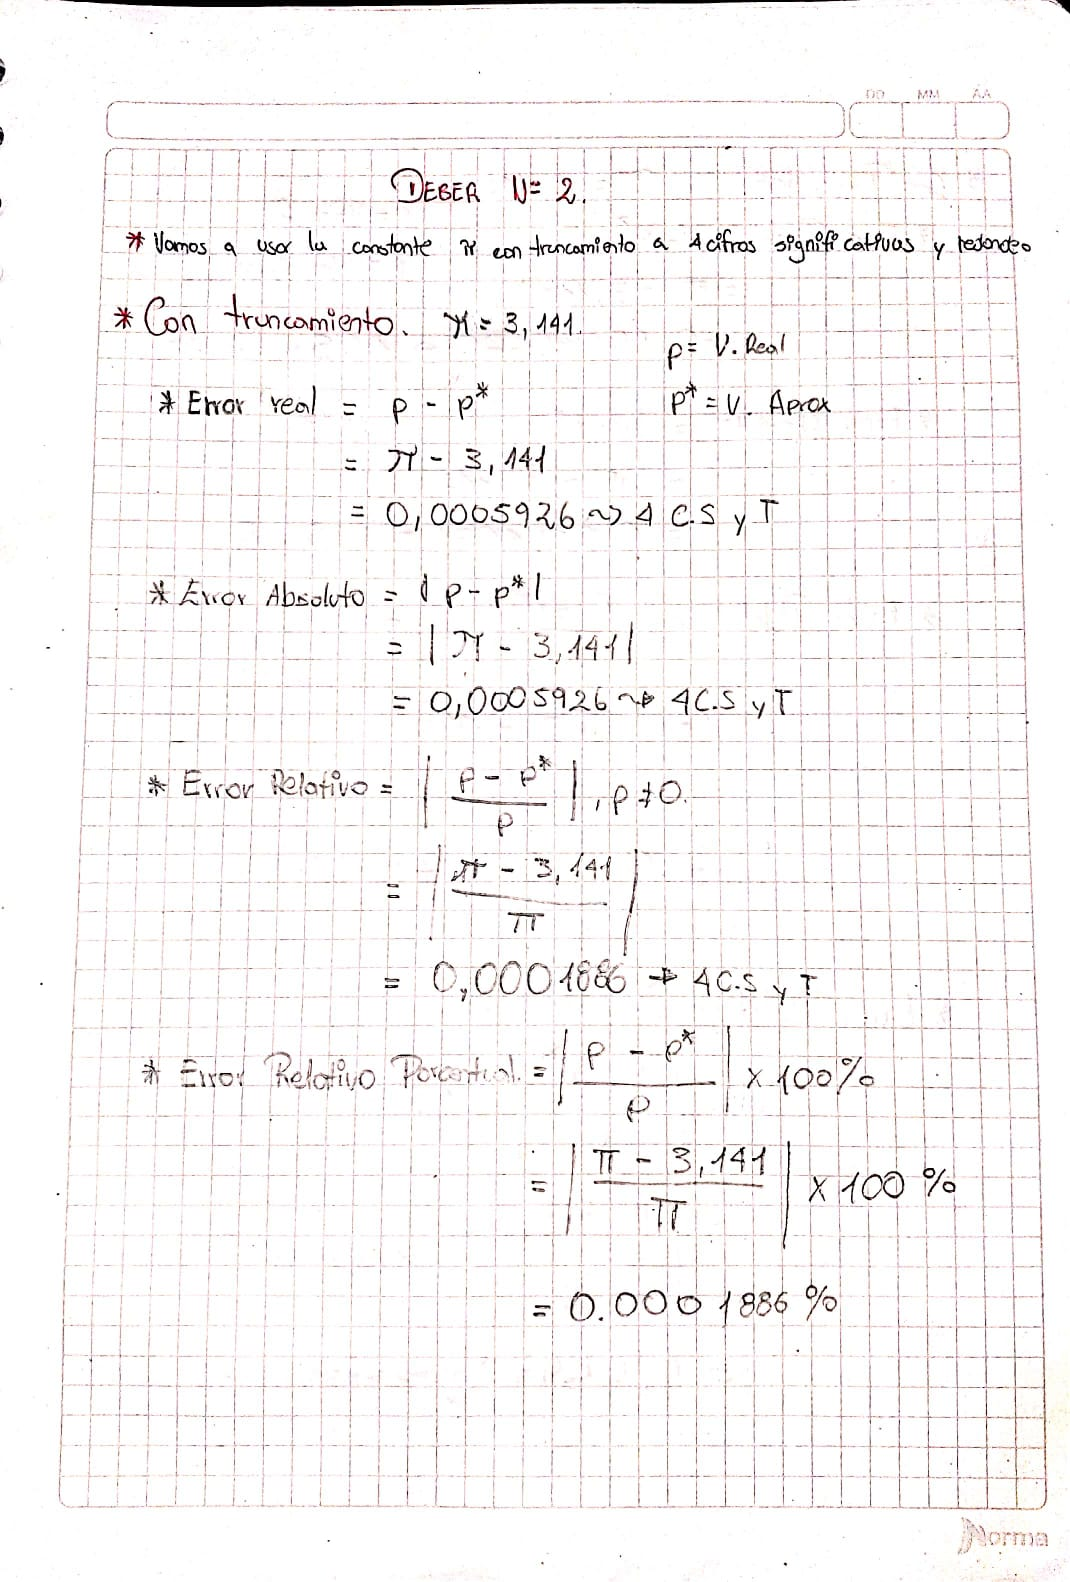
\includegraphics[width=0.95\textwidth]{inFiles/Figures/img1.jpeg}
\end{minipage}

\vspace{0.5cm}
\begin{minipage}{0.95\textwidth}
    \raggedleft
    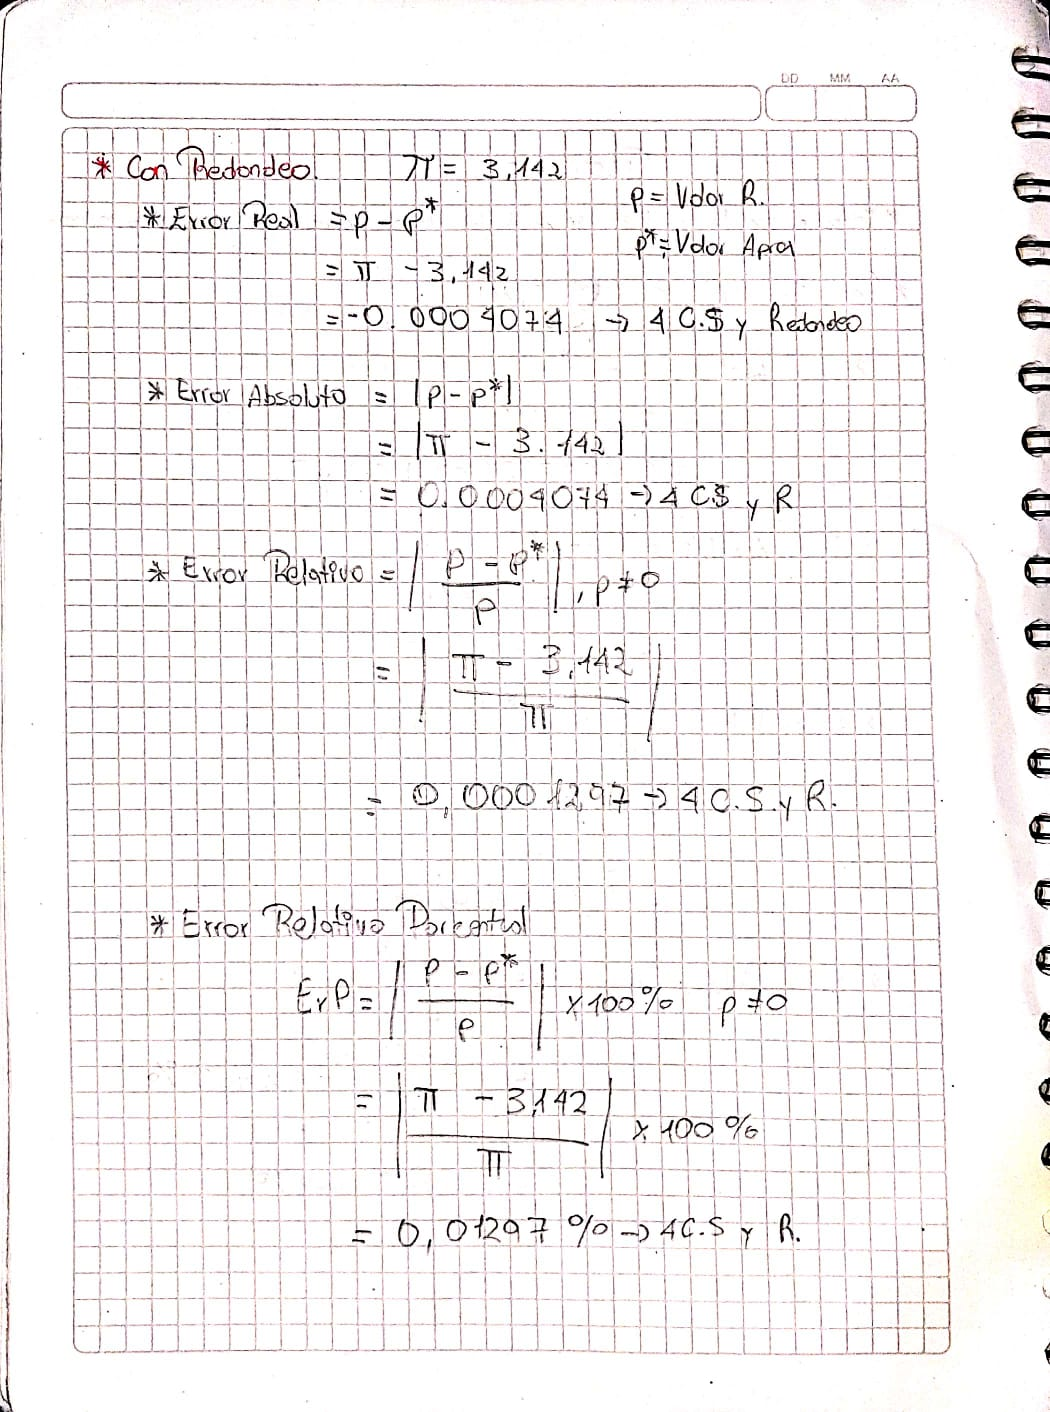
\includegraphics[width=0.95\textwidth]{inFiles/Figures/img2.jpeg}
\end{minipage}

\vspace{3cm}

\section*{CONCLUSIONES}
\begin{itemize}
    \item {Ambos métodos, truncamiento y redondeo son eficientes de diferentes
    formas ya que producen errores pequeños y son adecuados al momento de requerir
    precisión en los cálculos con cifras significativas relativamente pequeñas
    pero la que sobresale por su precisión al momento de compararlas es el método
    de redondeo.
    El análisis realizado nos muestra como los errores que se producen al momento de
    realizar cálculos numéricos son pequeños pero significativos al momento de requerir precisión
    en los valores obtenidos}
\end{itemize}


\vspace{0.5cm}


\end{document}
